\documentclass[10pt, compress]{beamer}

\usetheme{metropolis}           % Use metropolis theme

\usepackage[export]{adjustbox}
\usepackage{booktabs}
\usepackage[scale=2]{ccicons}
\usefonttheme[onlymath]{serif}

%\usemintedstyle{trac}

\title{A review of methods for Bayesian hierarchical clustering}
\subtitle{}
\date{June 3, 2016}
\author{Sharad Vikram}
\institute{UCSD}

%\setcounter{tocdepth}{1}

\begin{document}

\maketitle

\section{Background}

\subsection{Clustering}

\begin{frame}{Unsupervised learning}
  In unsupervised learning, we are interested in finding
        underlying structure
        in data.

  \pause
  Examples of unsupervised learning problems are:
 \metroset{block=fill}
  \begin{block}{Dimensionality reduction}
    Finding low-dimensional
      representations of high-dimensional data
  \end{block}
  \pause
 \metroset{block=fill}
  \begin{block}{Density estimation}
    Estimating an underlying probability distribution
    given samples from the distribution
  \end{block}
  \pause
 \metroset{block=fill}
  \begin{exampleblock}{Clustering}
    Discovering natural groups in data
  \end{exampleblock}
\end{frame}

\begin{frame}{Clustering}
  The most popular methods for clustering produce
  flat clusterings.

  A \alert{flat clustering} is a partition of a set of data,
  or an assignment of each data point into one of
  several disjoint sets.
  
  \pause

  \begin{align}
    \{1, 2, \ldots, N\} \rightarrow \{\{\ldots\}, \{\ldots\}, \ldots, \{\ldots\}\}
  \end{align}
\end{frame}

\begin{frame}{Flat clustering}
  The most popular algorithm for flat clustering is \alert{k-means}.
  \begin{enumerate}
    \item<2-> Pick a number of clusters $K$.
    \item<3-> Randomly initialize cluster centers $\{\mu_1, \ldots, \mu_K\}$.
    \item<4-> Alternate until convergence:
      \begin{itemize}
        \item Assign each data point to its closest cluster center.
        \item Assign each cluster center to the mean of its assigned data points.
      \end{itemize}
  \end{enumerate}
  \uncover<5->{
  This is equivalent to optimizing the loss function:
  \begin{align}
    L(\mu_1, \ldots, \mu_K) = \sum_{i = 1}^N \min_k \|x_i - \mu_k\|^2_2
  \end{align}}

  \only<6->{How do we pick $K$?}
\end{frame}

%\begin{frame}{Flat clustering: pros and cons}
  %\begin{table}
    %\begin{tabular}{lr}
      %\toprule
      %Pros & Cons \\
      %\midrule
      %Simple algorithms &  Requires specification of $k$ (in general)\\
      %Efficient algorithms & \\
      %Theoretical understanding & \\
      %\bottomrule
    %\end{tabular}
  %\end{table}
%\end{frame}

\begin{frame}{Hierarchical clustering}
  In \alert{hierarchical clustering}, data
  is recursively partitioned to form a tree (typically binary),
  also called a hierarchy.

  \begin{center}
    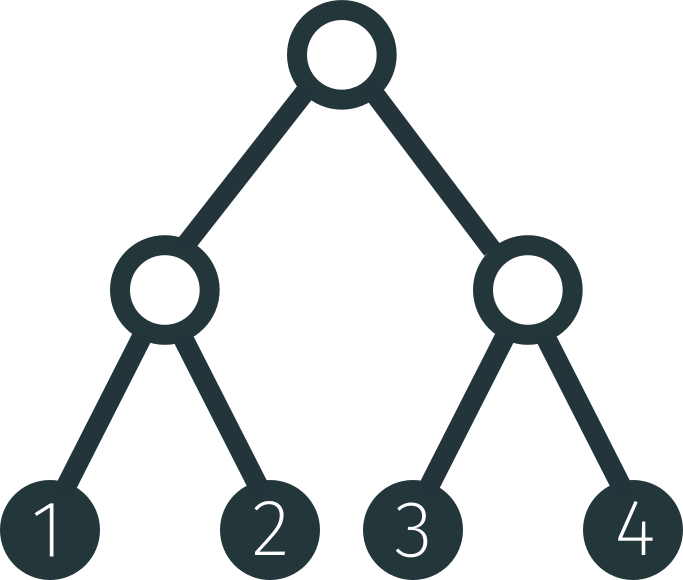
\includegraphics[width=0.5\textwidth]{img/tree-1234-balanced}
  \end{center}

  %\pause

  %Each leaf in the tree is a single data point,
  %The root is the grouping of all data points
  %into a single cluster and internal nodes
  %are groupings of different granularities.
\end{frame}

\begin{frame}{Traditional hierarchical clustering algorithms}
  Traditional clustering algorithms can be broadly broken
  down into two categories:

  \pause
 \metroset{block=fill}
  \begin{block}{Agglomerative (bottom-up)}
    The tree is built by
      beginning with just singleton clusters (leaves) and
      iteratively merging them until we have one cluster (root)
    \end{block}
  \pause
 \metroset{block=fill}
  \begin{block}{Divisive (top-down)}
    The tree is built
      by beginning with a single cluster (root) and
      recursively partitioning it until we
      have just singleton clusters (leaves)
  \end{block}
\end{frame}

%\begin{frame}{Agglomerative clustering}
  %The inputs to an agglomerative clustering algorithm
  %are:
  %\begin{itemize}
    %\item<2-> Dataset $X = \{x_i\}_{i = 1}^N$
    %\item<3-> Dissimilarity function $d(x, x')$
    %\item<4-> Linkage criterion $D(A, B)$.
  %\end{itemize}

%\end{frame}

%\begin{frame}{Dissimilarity functions}

  %A dissimilarity function measures how
  %different two data points are from each other.

  %\pause

 %\metroset{block=fill}
  %\begin{exampleblock}{Example dissimilarity functions}
  %\begin{itemize}
    %\item Euclidean distance: $d(x, x') = \|x - x'\|_2^2$
    %\item Manhattan distance: $d(x, x') = \|x - x'\|_1$
    %\item Mahalanobis distance: $d(x, x') = (x - x')^T\Sigma(x - x')$
  %\end{itemize}
  %\end{exampleblock}
%\end{frame}

%\begin{frame}{Linkage criteria}

  %A linkage measures how
  %different two \textbf{clusters} are from each other
  %in terms of dissimilarity function $d$.

  %\pause

 %\metroset{block=fill}
  %\begin{exampleblock}{Example linkage criteria}
  %\begin{itemize}
    %\item<2-> Single linkage: $D(A, B) = \min_{i \in A, j\in B} d(x_i, x_j)$
    %\item<3-> Complete linkage: $D(A, B) = \max_{i \in A, j\in B} d(x_i, x_j)$
    %\item<4-> Average linkage: $D(A, B) = \frac{1}{|A||B|}\sum_{i \in A, j\in B} d(x_i, x_j)$
  %\end{itemize}
  %\end{exampleblock}
%\end{frame}

\begin{frame}{Agglomerative clustering}
  We iteratively merge the two closest clusters until 
  we have one cluster left.

  \begin{center}
    \includegraphics<1>{img/agglomerative-clustering-0}
    \includegraphics<2>{img/agglomerative-clustering-1}
    \includegraphics<3>{img/agglomerative-clustering-2}
    \includegraphics<4>{img/agglomerative-clustering-3}

  \end{center}

  \begin{center}
    \only<1>{ $\{\{1\}, \{2\}, \{3\}, \{4\}\}$}
    \only<2>{ $\{\{1, 2\}, \{3\}, \{4\}\}$}
    \only<3>{ $\{\{1, 2\}, \{3, 4\}\}$}
    \only<4>{ $\{\{1, 2, 3, 4\}\}$}
  \end{center}
\end{frame}

\begin{frame}{Agglomerative clustering examples}
  \begin{figure}
    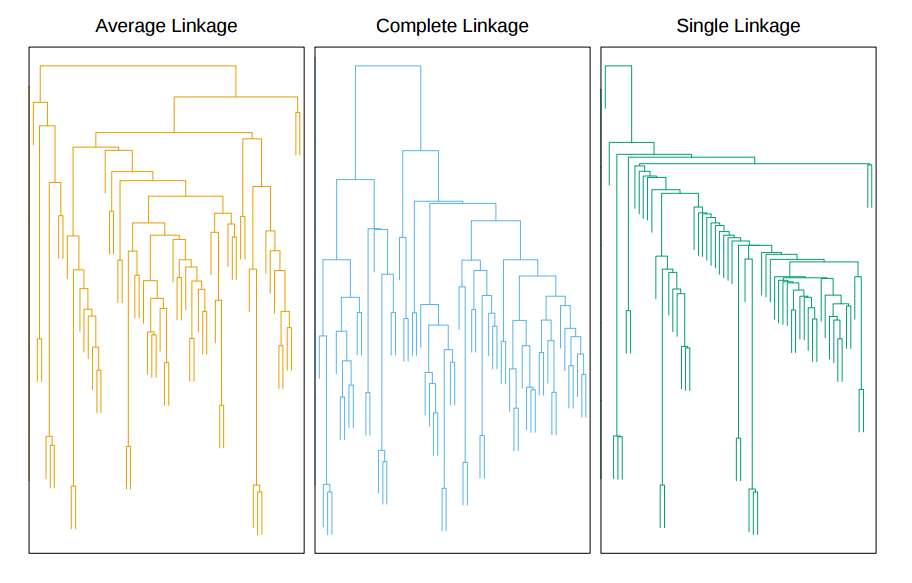
\includegraphics[frame,width=\textwidth]{img/dendrograms}
    \caption{Trees produced by agglomerative clustering algorithms
    with different linkage criteria. Source: \cite{Hastie2009}}
    \label{fig:dendrograms}
  \end{figure}
\end{frame}

\begin{frame}{Divisive clustering}
  In divisive clustering, we begin with the root cluster
  and recursively partition it until we are left with
  singleton leaf clusters.

 \metroset{block=fill}
  \begin{block}{Approaches}
    \begin{itemize}
    \item Use $k$-means recursively until only singleton clusters
    \item Define a similarity graph $G$ in terms of similarity function $s(x, x')$
      and perform partitions by finding a minimum cut on $G$.
    \end{itemize}
  \end{block}
\end{frame}

\begin{frame}{Ambiguous data}
  Consider the two following scenarios where
  circles represent tight clusters of data.

  \begin{center}
  \includegraphics[width=0.3\textwidth]{img/3-cluster}\hfill
  
\includegraphics[width=0.45\textwidth]{img/3-cluster-line}
  \end{center}

  \pause

  A single binary tree is not sufficient to describe either
  of these configurations.

  %\centering
  %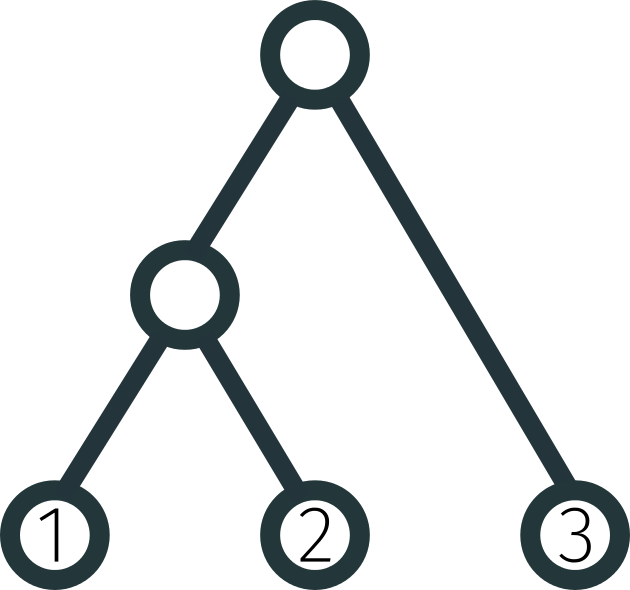
\includegraphics[width=0.3\textwidth]{img/tree-123} \hfill
  %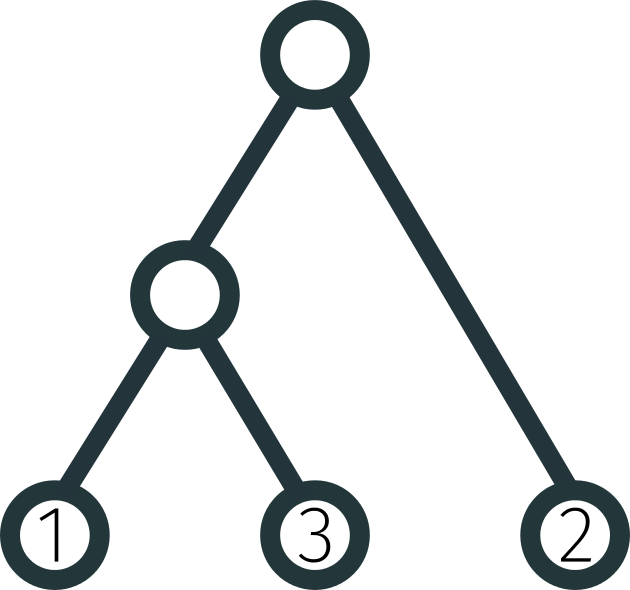
\includegraphics[width=0.3\textwidth]{img/tree-132} \hfill
  %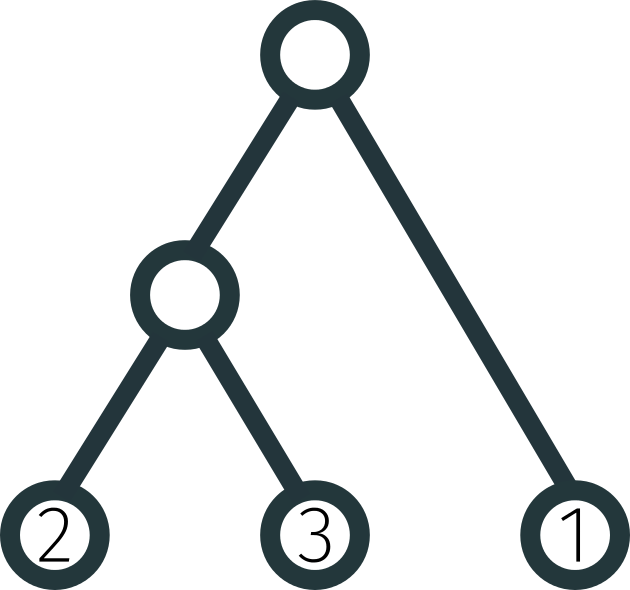
\includegraphics[width=0.3\textwidth]{img/tree-231}

\end{frame}

\begin{frame}{Multifurcating trees}
  Perhaps extending our binary trees to $k$-ary trees will help.

  \begin{center}
    \includegraphics<1>[width=0.8\textwidth]{img/3-cluster-both.png}
    \includegraphics<2>[width=0.8\textwidth]{img/3-cluster-both-2.png}
    \includegraphics<3>[width=0.8\textwidth]{img/3-cluster-both-3.png}
  \end{center}

\end{frame}

\begin{frame}{Uncertainty in hierarchies}
  Furthermore, small perturbations in our data
  can have an effect on the output
  hierarchy.

  \begin{center}
    \includegraphics<1>[width=0.8\textwidth]{img/3-cluster-line-noperturb}
    \includegraphics<2->[width=0.8\textwidth]{img/3-cluster-line-perturb}
  \end{center}

  %\uncover<3>{We need a more general approach.}
\end{frame}

\begin{frame}{Probabilistic reasoning}
  One approach is to
  model ambiguity and uncertainty with \textbf{probability}.
  We output a probability distribution over all possible
  trees.

  \begin{center}
    \includegraphics<2>[width=0.7\textwidth]{img/3-cluster-distribution.png}
    \includegraphics<3>[width=0.7\textwidth]{img/3-cluster-linear-distribution.png}
  \end{center}
\end{frame}

\subsection{Bayesian learning}

\begin{frame}{Latent variable models}
  We take a quick detour to review Bayesian learning.
  \begin{center}
    \includegraphics<2>[width=0.1\textwidth]{img/latent-variable-model-0}
    \includegraphics<3->[width=0.1\textwidth]{img/latent-variable-model}
  \end{center}
\uncover<4->{
  Our data $X$ is generated conditionally given a set of
  unobserved \alert{latent} variables $\theta$.
}
\end{frame}

\begin{frame}{Distributions of interest}
  We are interested in the \alert{posterior distribution}
  of latent variables given data, $P(\theta | X)$,
  calculated via Bayes rule.
  \pause

  \begin{align}
    P(\theta | X) = \frac{P(X | \theta)P(\theta)}{P(X)} = \frac{P(X | \theta)P(\theta)}{\int_\Theta P(X|\theta)P(\theta)d\theta}
  \end{align}
  \pause
  $P(\theta)$ is called the \alert{prior distribution} and $P(X|\theta)$ is called the
  \alert{likelihood model}. They are specified beforehand.
\end{frame}

\begin{frame}{Bayesian inference}
  Typically the hardest part of computing the
  the posterior distribution is calculating
  $P(X) = \int_\Theta P(X|\theta)P(\theta)d\theta$, the \alert{marginal distribution}.

   \pause 

  When the prior $P(\theta)$ and likelihood $P(X|\theta)$ are
  conjugate, the posterior is analytically computable.

  \pause

  Otherwise, we usually approximate it with methods such as:
  \begin{itemize}
    %\item Loopy belief propagation
    \item Markov chain Monte Carlo (MCMC)
    \item Variational inference
    \item MAP estimation via EM
  \end{itemize}
\end{frame}

\section{Bayesian hierarchical clustering}

\begin{frame}{BHC as a latent variable model}
  Bayesian hierarchical clustering is a
  statistical approach, specifically
  a \alert{latent variable model}.
  \pause
  \begin{center}
    \includegraphics[width=0.3\textwidth]{img/bhc-lvm}
  \end{center}
  It is composed of data $X$ and
  latent variables $T$ and $\theta$.
  \pause
  \begin{itemize}
    \item $T$ is a tree structure, sampled from a \alert{tree prior} distribution $P(T)$.
    \item $\theta$ is a set of parameters, generated in a \alert{tree likelihood} model $P(\theta | T)$.
  \end{itemize}
\end{frame}

\begin{frame}{Tree priors}
  Most often we are interested in rooted binary trees with labeled leaves,
  also called \alert{cladograms}.

  \begin{center}
    \includegraphics<1>[width=0.4\textwidth]{img/tree-4}
    \includegraphics<2>[width=0.4\textwidth]{img/tree-4-ordering}
    \includegraphics<3>[width=0.4\textwidth]{img/tree-4-ordering-times}
  \end{center}

  Very often, cladograms will contain additional information.

  \begin{itemize}
    \item<2-> An ordering on the internal nodes
    \item<3-> Times associated with each node
  \end{itemize}

\end{frame}

\begin{frame}{Tree priors}
  The simplest tree prior is the uniform distribution over
  cladograms.

  \pause

  \begin{center}
    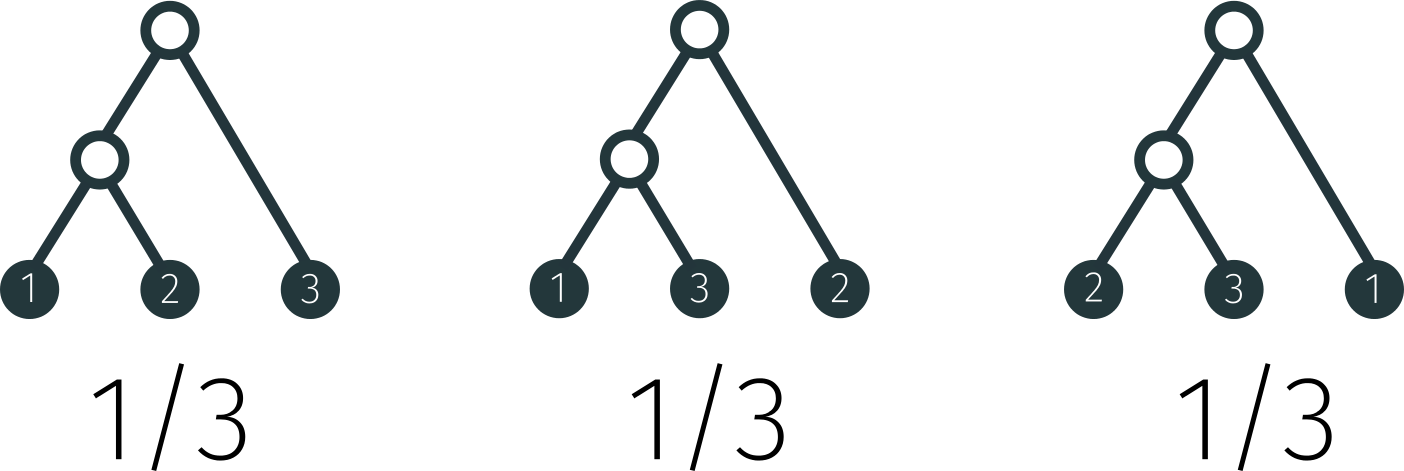
\includegraphics[width=0.6\textwidth]{img/uniform-distribution}
  \end{center}

  \pause
  In general, however, tree priors mostly fall into two categories:
 \metroset{block=fill}
  \begin{block}{Coalescent models}
    Trees are modeled in an
      agglomerative fashion, merging clusters until 
      one is left
    \end{block}
  \begin{block}{Diffusion models}
    Trees are modeled inductively,
      starting with a tree of size $1$ and growing it to
      a tree of size $N$.
    \end{block}
\end{frame}

\subsection{Coalescent models}

\begin{frame}{Coalescent models}
  Coalescent models begin with a set of $N$
  data, or "individuals", at $t = 0$.

  \begin{center}
    \includegraphics<1>[width=0.5\textwidth]{img/coalescent-1}
    \includegraphics<2>[width=0.5\textwidth]{img/coalescent-2}
    \includegraphics<3>[width=0.5\textwidth]{img/coalescent-3}
    \includegraphics<4>[width=0.5\textwidth]{img/coalescent-4}
  \end{center}

  \pause

  Every iteration, we:
  \begin{itemize}
    \item Pick two distinct nodes $a$ and $b$ uniformly at random.
    \item Sample a coalesce time $t$.
    \item Create an internal node whose children are $a$ and $b$
      with time $t$.
  \end{itemize}
\end{frame}


\begin{frame}{Kingman's coalescent}
  The simplest coalescent model is \alert{Kingman's coalescent} \cite{Kingman1982},
  where we assume a constant coalesce rate.

  There are a total of
  $N - 1$ events happening at time $t_{N - 1} < t_{N - 2} < \cdots < t_1$.

  \pause

  \begin{center}
    \includegraphics[width=\textwidth]{img/coalescent-times}
  \end{center}


    Let $\delta_i$ represent the elapsed time
  between coalescent event $i-1$ and $i$.
  We let
  \begin{align}
    \delta_i \sim \mathrm{Exp}\left(\binom{N - i + 1}{2}\right)
  \end{align}

\end{frame}

\begin{frame}{Kingman's coalescent}
  \begin{itemize}
    \item<1-> Kingman's coalescent corresponds
  to the uniform distribution
  over \emph{ordered cladograms}.

    \item<2-> Its induced distribution over
  unordered cladograms is the time-marginalized coalescent (TMC) \cite{Boyles2012}.

    \item<3-> What sort of trees does Kingman's coalescent favor?
      \begin{center}
        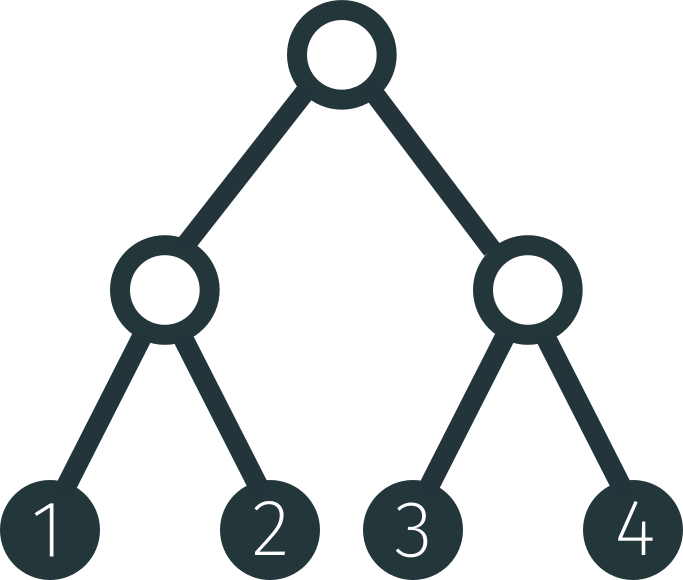
\includegraphics[width=0.4\textwidth]{img/tree-1234-balanced} \hspace{0.4em}
        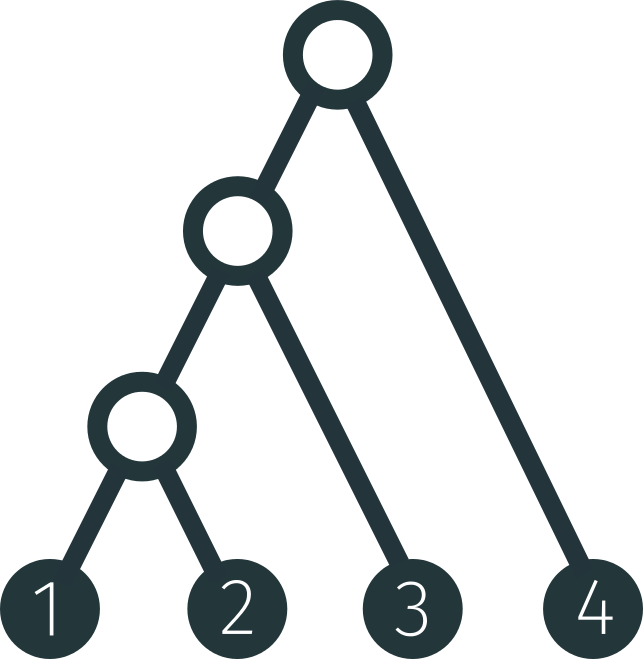
\includegraphics[width=0.37\textwidth]{img/tree-4-unbalanced}
      \end{center}
  \end{itemize}
\end{frame}

\begin{frame}{Time-marginalized coalescent}
  \begin{itemize}
    \item<1->Kingman's coalescent produces
  cladograms with ordering and times.


  \item<2->Marginalizing out the time is easy, since it's
    generated independently. Node ordering
    is not so easy.

\item<3-> The number of possible node orderings for a given unordered
  binary tree with $N$ leaves is

  \begin{align}
    \frac{(N - 1)!}{\prod_{i = 1}^{N - 1} m_i}
  \end{align}

  where $m_i$ is the number of internal nodes in the subtree indexed by $i$.
  \end{itemize}
\end{frame}

\begin{frame}{TMC vs. Kingman's coalescent}

  Consider an ordered cladogram $\phi$
  and an unordered cladogram $\psi$, both with $N$ leaves.

  \begin{itemize}
    \item<1-> Kingman's coalescent induces the uniform
    distribution over ordered cladograms.
    \begin{align*}
      P(\phi) = \left(\prod_{i = 1}^{N}\binom{i}{2}\right)^{-1}
    \end{align*}
    \item<2-> The TMC is the induced
    distribution over unordered cladograms.
    \begin{align*}
      P(\psi) = \frac{(N - 1)!}{\prod_{i = 1}^{N - 1} m_i} \left(\prod_{i = 1}^{N}\binom{i}{2}\right)^{-1}
    \end{align*}
    \item<3-> Kingman's coalescent
      and TMC favor balanced trees!
  \end{itemize}
\end{frame}

\begin{frame}{The $\Lambda$-coalescent}
  \begin{itemize}
    \item<1-> The $\Lambda$-coalescent generalizes Kingman's coalescent
      to both multifurcating trees and more complex
      distributions over times \cite{Pitman1999}.

    \item<2-> Rather than 
      $\delta_i \sim \mathrm{Exp}\left(\binom{N - i + 1}{2}\right)$,
      we have
      \begin{align}
        \lambda_i^k &= \int_0^1 \gamma^{k - 2}(1 - \gamma)^{(i-k)}\Lambda(d\gamma)\\
        \delta_i &\sim \mathrm{Exp}\left(\lambda_i^k\right),
      \end{align}
      for finite measure $\Lambda$ and max branching factor $k$.
    \item<3-> When $\Lambda$ is the Dirac delta and $k = 2$,
      we have Kingman's coalescent.

  \end{itemize}
\end{frame}

\subsection{Diffusion models}

\begin{frame}{Diffusion models}
  Basic idea: begin with a tree over
    one data, then for $N$ iterations:
  \begin{itemize}
    \item Sample a branch and time at random.
    \item Attach a leaf to the branch,
      creating a new internal node with the sampled time.
  \end{itemize}
  \begin{center}
    \includegraphics<2>[width=\textwidth]{img/diffusion-1}
    \includegraphics<3>[width=\textwidth]{img/diffusion-2}
    \includegraphics<4>[width=\textwidth]{img/diffusion-3}
    \includegraphics<5>[width=\textwidth]{img/diffusion-4}
  \end{center}
\end{frame}

\begin{frame}{Dirichlet diffusion tree}
    The simplest model is the Dirichlet diffusion tree (DDT),
    which produces trees with both ordering
    and times associated with internal nodes \cite{Neal2003}.

    The model is defined inductively via a continuous time
    process. Assume we have a tree of size $i - 1$.

    \pause

    \begin{center}
      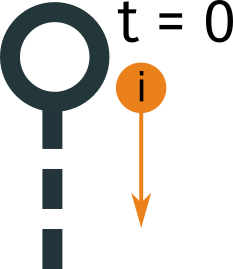
\includegraphics[width=0.2\textwidth]{img/ddt-1}
    \end{center}

    On each iteration, a particle labeled $i$ begins at the root and travels downwards.
\end{frame}

\begin{frame}{Dirichlet diffusion tree}
  \textbf{Case 1:} 
  The particle reaches an internal node.
  \begin{center}
      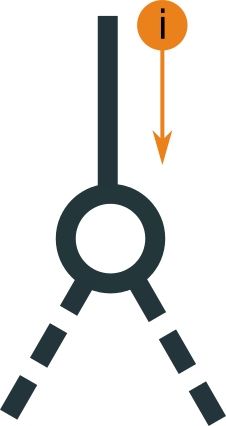
\includegraphics[width=0.13\textwidth]{img/ddt-2}
  \end{center}

  \pause

  It picks one of the branches proportional to the past number
  of particles that have picked either branch.

  \pause

  \begin{center}
      \includegraphics[width=0.17\textwidth]{img/ddt-3}
  \end{center}
\end{frame}

\begin{frame}{Dirichlet diffusion tree}
  \textbf{Case 2:} 
  The particle \emph{diverges} on its current branch,
  creating an internal node and a leaf.
  The probability of divergence is calculated from
  an \alert{acquisition function}, $a(t)$.


  \begin{center}
      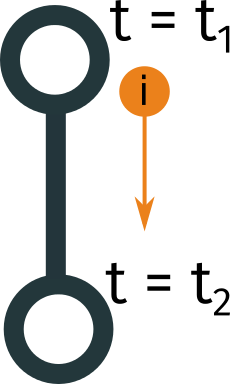
\includegraphics[width=0.09\textwidth]{img/ddt-4}
  \end{center}

  \pause

  Let $m$ be the number of past particles that have traversed the current branch.
  The probability of diverging at time $dt$ is $a(t)dt/m$.

  \pause

  \begin{center}
      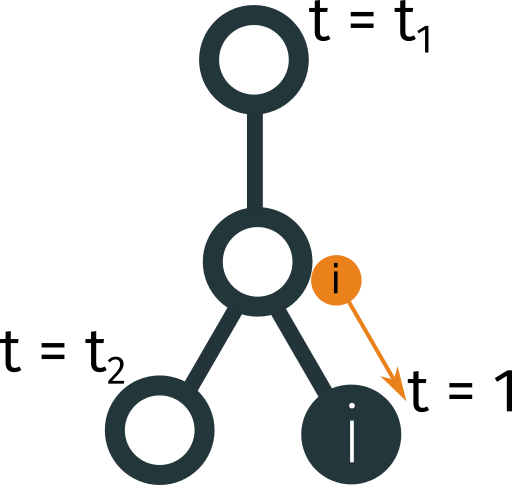
\includegraphics[width=0.18\textwidth]{img/ddt-5}
  \end{center}

  \pause

  If $a(1) = \infty$, each particle is guaranteed to diverge before $t = 1$.

\end{frame}

\begin{frame}{Pitman-Yor diffusion tree}
  The DDT has been extended to
  multifurcating trees with the Pitman-Yor diffusion tree (PYDT) \cite{Knowles2015}.

  The $i$-th particle behaves slightly differently, but
  starts in the same way.

  \begin{center}
      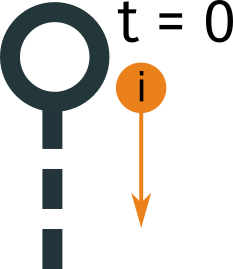
\includegraphics[width=0.15\textwidth]{img/ddt-1}
  \end{center}

\end{frame}

\begin{frame}{Pitman-Yor diffusion tree}
  \textbf{Case 1:} 
  The particle reaches an internal node that has $b$ branches already.
  \begin{center}
      \includegraphics[width=0.13\textwidth]{img/pydt-1}
  \end{center}

  \pause

  It picks the $k$-th branch with probability
  \begin{align}
      \frac{m_k - \beta}{m + \alpha}
  \end{align}
  where $m_k$ is the number of past particles that have traversed the $k$-th branch,
  $m$ is the total number of particles that have traversed this subtree,
  and $\alpha$ and $\beta$ are hyperparameters.

\end{frame}

\begin{frame}{Pitman-Yor diffusion tree}
  \textbf{Case 2:} 
  The particle reaches an internal node that has $b$ branches already.
  \begin{center}
      \includegraphics[width=0.13\textwidth]{img/pydt-1}
  \end{center}

  \pause

  It creates a new branch with probability
  \begin{align}
      \frac{\alpha + \beta b}{m + \alpha}
  \end{align}

\end{frame}

\begin{frame}{Pitman-Yor diffusion tree}
  \textbf{Case 3:} 
  The particle \emph{diverges} on its current branch,
  creating an internal node and a leaf.
  The probability of divergence is calculated from
  an \alert{acquisition function}, $a(t)$.

  \begin{center}
      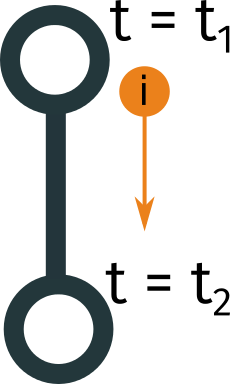
\includegraphics[width=0.09\textwidth]{img/ddt-4}
  \end{center}

  \pause

  Let $m$ be the number of past particles that have traversed the current branch.
  The probability of diverging at time $dt$ is

  \pause

  \begin{align}
    \frac{a(t)\Gamma(m - \beta)dt}{\Gamma(m + 1 + \alpha)}
  \end{align}

\end{frame}

\begin{frame}{Generalizations}
  \begin{center}
    \includegraphics<1>[width=0.8\textwidth]{img/tree-graph-0}
    \includegraphics<2>[width=0.8\textwidth]{img/tree-graph-1}
    \includegraphics<3>[width=0.8\textwidth]{img/tree-graph-2}
    \includegraphics<4>[width=0.8\textwidth]{img/tree-graph-3}
    \includegraphics<5>[width=0.8\textwidth]{img/tree-graph-4}
    \includegraphics<6>[width=0.8\textwidth]{img/tree-graph-5}
    \includegraphics<7>[width=0.8\textwidth]{img/tree-graph-6}
    \includegraphics<8>[width=0.8\textwidth]{img/tree-graph-7}
  \end{center}
\end{frame}

\begin{frame}{Tree likelihood models}
  Now, given a sample from a tree prior (assume a
  cladogram with ordering and times),
  we need to generate a dataset.

  \begin{center}
    \includegraphics<1>[width=\textwidth]{img/tree-data-0}
    \includegraphics<2>[width=\textwidth]{img/tree-data-1}
  \end{center}

\end{frame}

\begin{frame}{Latent tree parameters}
  For every internal node in the tree $n$
  we associate a latent parameter $\theta_n$
  which is in the same space as the data.

  \begin{center}
    \includegraphics<2->[width=0.35\textwidth]{img/tree-4-parameters}
  \end{center}

  \pause

  We then define:
  \begin{itemize}
    \item<3-> A prior distribution $P_0(\theta)$ from which $\theta_0$ is generated
    \item<4-> A transition kernel $T(\theta' | \theta)$ that describes a Markov
      process beginning at the root. Each parameter $\theta'$ is generated
      conditioned solely on its parent $\theta$. In addition, leaves are generated
      conditioned on their parent.
  \end{itemize}

\end{frame}

\begin{frame}{Example likelihood models}
  The most common likelihood model is \alert{Brownian motion},
  also called Gaussian diffusion, which is
  \begin{align}
    P_0(\theta) &= \mathcal{N}(0, \sigma_0^2I) \\
    T(\theta' | \theta) &= \mathcal{N}(\theta, \sigma^2(t - t')),
  \end{align}
  where $t$ and $t'$ are the times associated with nodes
  $\theta$ and $\theta'$ and $\sigma_0^2$ and $\sigma^2$ are hyperparameters.

  \pause

  Other options are:
  \begin{itemize}
    \item Multinomial-Dirichlet diffusion: useful for
      categorical data
    \item Multinomial diffusion: useful for
      counts (such as bag-of-words)
  \end{itemize}
\end{frame}

\subsection{Inference}
\begin{frame}{Inference}
  Recall the latent variable model.
  \begin{center}
    \includegraphics[width=0.3\textwidth]{img/bhc-lvm}
  \end{center}
  \pause

  We are interested in computing the posterior distribution
  $P(T, \theta | X)$ and the posterior marginal distribution
  $P(T | X)$.

  \pause

  Both of these distributions are generally impossible
  to write out analytically, so we use approximate methods.
  In this report, we'll focus on a particular sampling method.
\end{frame}

\begin{frame}{Metropolis-Hastings}
  
  The \alert{Metropolis-Hastings} (MH) algorithm
  is an MCMC method that uses
  samples from a distribution $p(x)$ to approximate it.

  \pause
 \metroset{block=fill}
  \begin{block}{Metropolis-Hastings algorithm}
  \begin{itemize}
    \item Given initial distribution $p_0(x)$ and proposal distribution
      $q(x'|x)$
    \item Instantiate $x_0$ by sampling $p_0(x)$.
      \pause
    \item Repeat for $t = 1 \ldots T$
      \pause
      \begin{itemize}
        \item Sample $x'$ from $q(x'|x_{t - 1})$.
      \pause
        \item Calculate acceptance ratio
          \begin{align}
              \alpha = \frac{p(x')q(x_t | x')}{p(x_t)q(x' | x_t)}
          \end{align}
      \pause
        \item If $\alpha > 1$, accept the sample, setting $x_t = x'$
      \pause
        \item If $\alpha \le 1$, accept $x'$ with probability $\alpha$
          and reject otherwise, setting $x_t = x_{t - 1}$.
      \end{itemize}
  \end{itemize}
\end{block}
  \pause
  We now have samples $x_0, \ldots, x_T$.
\end{frame}

\begin{frame}{Sampling latent variables}
  Recall that we are interested in $P(T, \theta | X)$.
  To sample from the posterior using MH,
  we need to define a proposal distribution
  $q(T', \theta' | T, \theta)$ and an initial distribution $p_0(T, \theta)$.
  \begin{itemize}
    \item<2-> $p_0(T, \theta)$ is easy: just sample the tree prior
      and the tree likelihood model
    \item<3-> $q(T', \theta'| T, \theta)$ can be decoupled
      into two proposals: a 
      tree proposal $q_\mathcal{T}(T' | T)$
      and parameter proposal $q_\Theta(\theta' | T', \theta)$.
  \end{itemize}
\end{frame}

\begin{frame}{Subtree-prune and regraft}
  The \alert{subtree-prune and regraft} (SPR) move
  is a popular tree proposal distribution.

  An SPR move consists of a \emph{prune} and a \emph{regraft}.

  \begin{center}
    \includegraphics<2>[width=\textwidth]{img/spr-1}
    \includegraphics<3>[width=\textwidth]{img/spr-2}
    \includegraphics<4>[width=\textwidth]{img/spr-3}
  \end{center}

  \pause

  Let $T$ be a tree, $s$ be a non-root node in $T$ selected randomly and $S$ be its associated subtree.
  \begin{itemize}
    \item<3->
      We first prune
      $S$ from $T$ by
      remove $s$'s parent $p$ from the tree,
      replacing $p$ with $s$'s sibling.
    \item<4-> We then 
      regraft $p$ to $T$,
      by first randomly selecting a branch in $T$,
      and attaching $s$ to the branch.
  \end{itemize}
\end{frame}


\begin{frame}{Sampling latent parameters}
  We now have $q_\mathcal{T}(T' | T)$, the tree proposal distribution
   and have several options for the parameter proposal distribution:

   \begin{itemize}
     \item<2-> \textbf{Gibbs sampling:} since the parameters are generated
       in a Markovian process, the conditional distributions are often
       easy to compute
     \item<3-> \textbf{Marginalization via belief propagation:} if we're not
       interested in the parameters at all, we can marginalize them out
       and just sample tree structure via the tree proposal distribution
     \item<3-> \textbf{Other MCMC methods:} examples are slice sampling,
       and sequential Monte Carlo
   \end{itemize}
\end{frame}

\section{Adding interaction}

\begin{frame}{Why interaction?}
  Recall the motivating example for Bayesian hierarchical clustering.
  \begin{center}
  \includegraphics[width=0.3\textwidth]{img/3-cluster}\hfill
  
\includegraphics[width=0.45\textwidth]{img/3-cluster-line}
  \end{center}
  Could a user provide feedback and help decide which hierarchy
  makes the most sense?
  \begin{itemize}
    \item Interactive Bayesian Hierarchical Clustering - Vikram and Dasgupta (2016) \cite{Vikram2016}
  \end{itemize}
\end{frame}

\begin{frame}{Interactive hierarchical clustering}
  We first consider \emph{how} the user interacts
  with the algorithm.

  We propose the user provides feedback in the form
  of a \alert{triplet} of leaves $(\{a, b\}, c)$, which stipulates
  that $a$ must be in a subtree with $b$ that does not
  include $c$.

 \metroset{block=fill}
  \begin{block}{Simple method}
    \begin{itemize}
      \item Run a hierarchical clustering algorithm to obtain tree $T$.
      \item Repeat:
        \begin{itemize}
          \item Show $T$ to a user and they will return a triplet that is violated by $T$.
          \item Fix $T$ to not violate the triplet.
        \end{itemize}
    \end{itemize}
  \end{block}

  This is difficult for a user to do if the tree is too big!

\end{frame}

\begin{frame}{Subtree queries}
  We propose \alert{subtree queries}. Rather than showing
  the user the entire hierarchy $T$, we select a subset of data $S$
  and show the user the hierarchy
  restricted to a subset of the data, $T|_S$.

  \pause

 \metroset{block=fill}
  \begin{block}{Subtree querying method}
  \begin{itemize}
    \item Run a hierarchical clustering algorithm to obtain tree $T$.
    \item Repeat:
      \begin{itemize}
        \item Select subset $S$ of the data.
        \item Show $T|_S$ to a user 
          and they will return a triplet that is violated by $T|_S$.
        \item Fix $T$ to not violate the triplet.
      \end{itemize}
  \end{itemize}
  \end{block}

  \pause
  We now need to specify methods to
  \begin{itemize}
    \item Enforce triplet constraints in a clustering algorithm
    \item Select subsets to show the user
  \end{itemize}
  Bayesian learning provides
  elegant ways to design such methods.
\end{frame}


\begin{frame}{Enforcing triplet constraints}
  We can easily enforce triplet constraints
  in Bayesian hierarchical clustering.

  During inference, we use MH with a modified SPR proposal called
  the constrained-SPR proposal which will
  only select regraft branches
  that don't violate a set of
  triplet constraints.

    \pause

  \begin{center}
    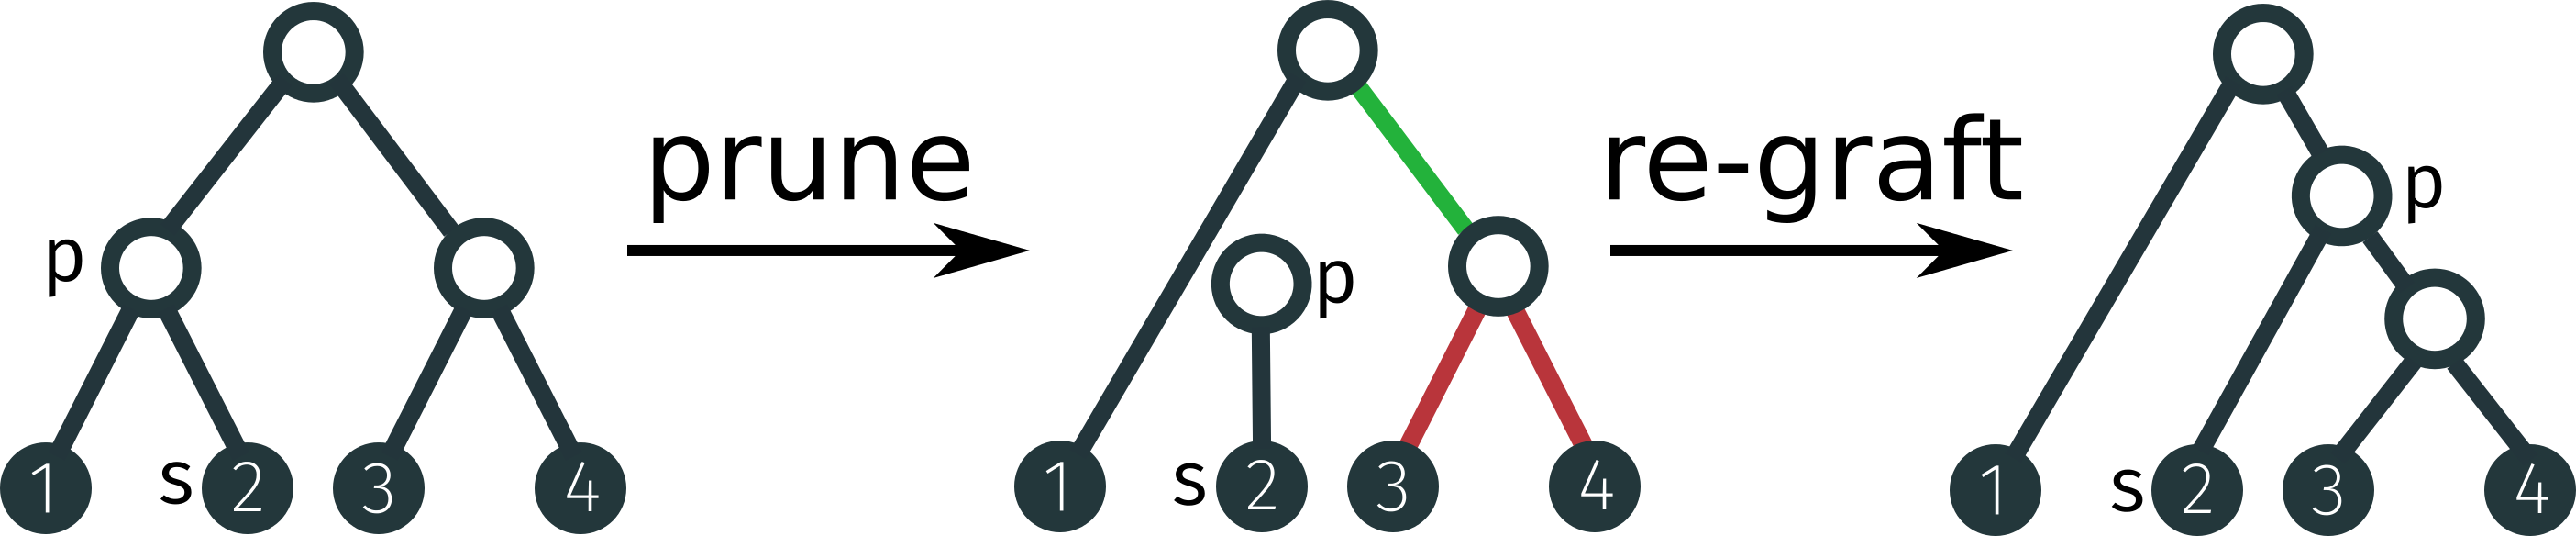
\includegraphics[width=\textwidth]{img/cspr-animation}
  \end{center}
\end{frame}

\begin{frame}{Intelligent subset queries}
  The simplest way to select a subset of data
  to show the user is random selection,
  we can use the Bayesian framework to choose better subsets.

  In BHC, we compute a posterior distribution over
  trees given data. Using the posterior,
  we can estimate the variance
  of various regions of the tree and show the
  user the region with the most variance.

 \metroset{block=fill}
  \begin{block}{Definition: tree distance variance (TDV)}
    Given a subset of data $S$ and tree samples $\mathcal{T} = T_1, \ldots, T_N$,
    \begin{align}
      \mathrm{TDV}(S, \mathcal{T}) = \max_{i, j \in S}  \mathrm{Var}_{T \in \mathcal{T}}\left[\texttt{tree-dist}_{T|S}(i, j)\right]
    \end{align}
  where $\texttt{tree-dist}_T$ is the number of edges needed to get from leaf $i$ to leaf $j$
  in tree $T$.
  \end{block}

  We now instantiate several random subsets and show the user the one with the highest TDV.
\end{frame}

\begin{frame}{Results}
  \begin{figure}
    \centering
    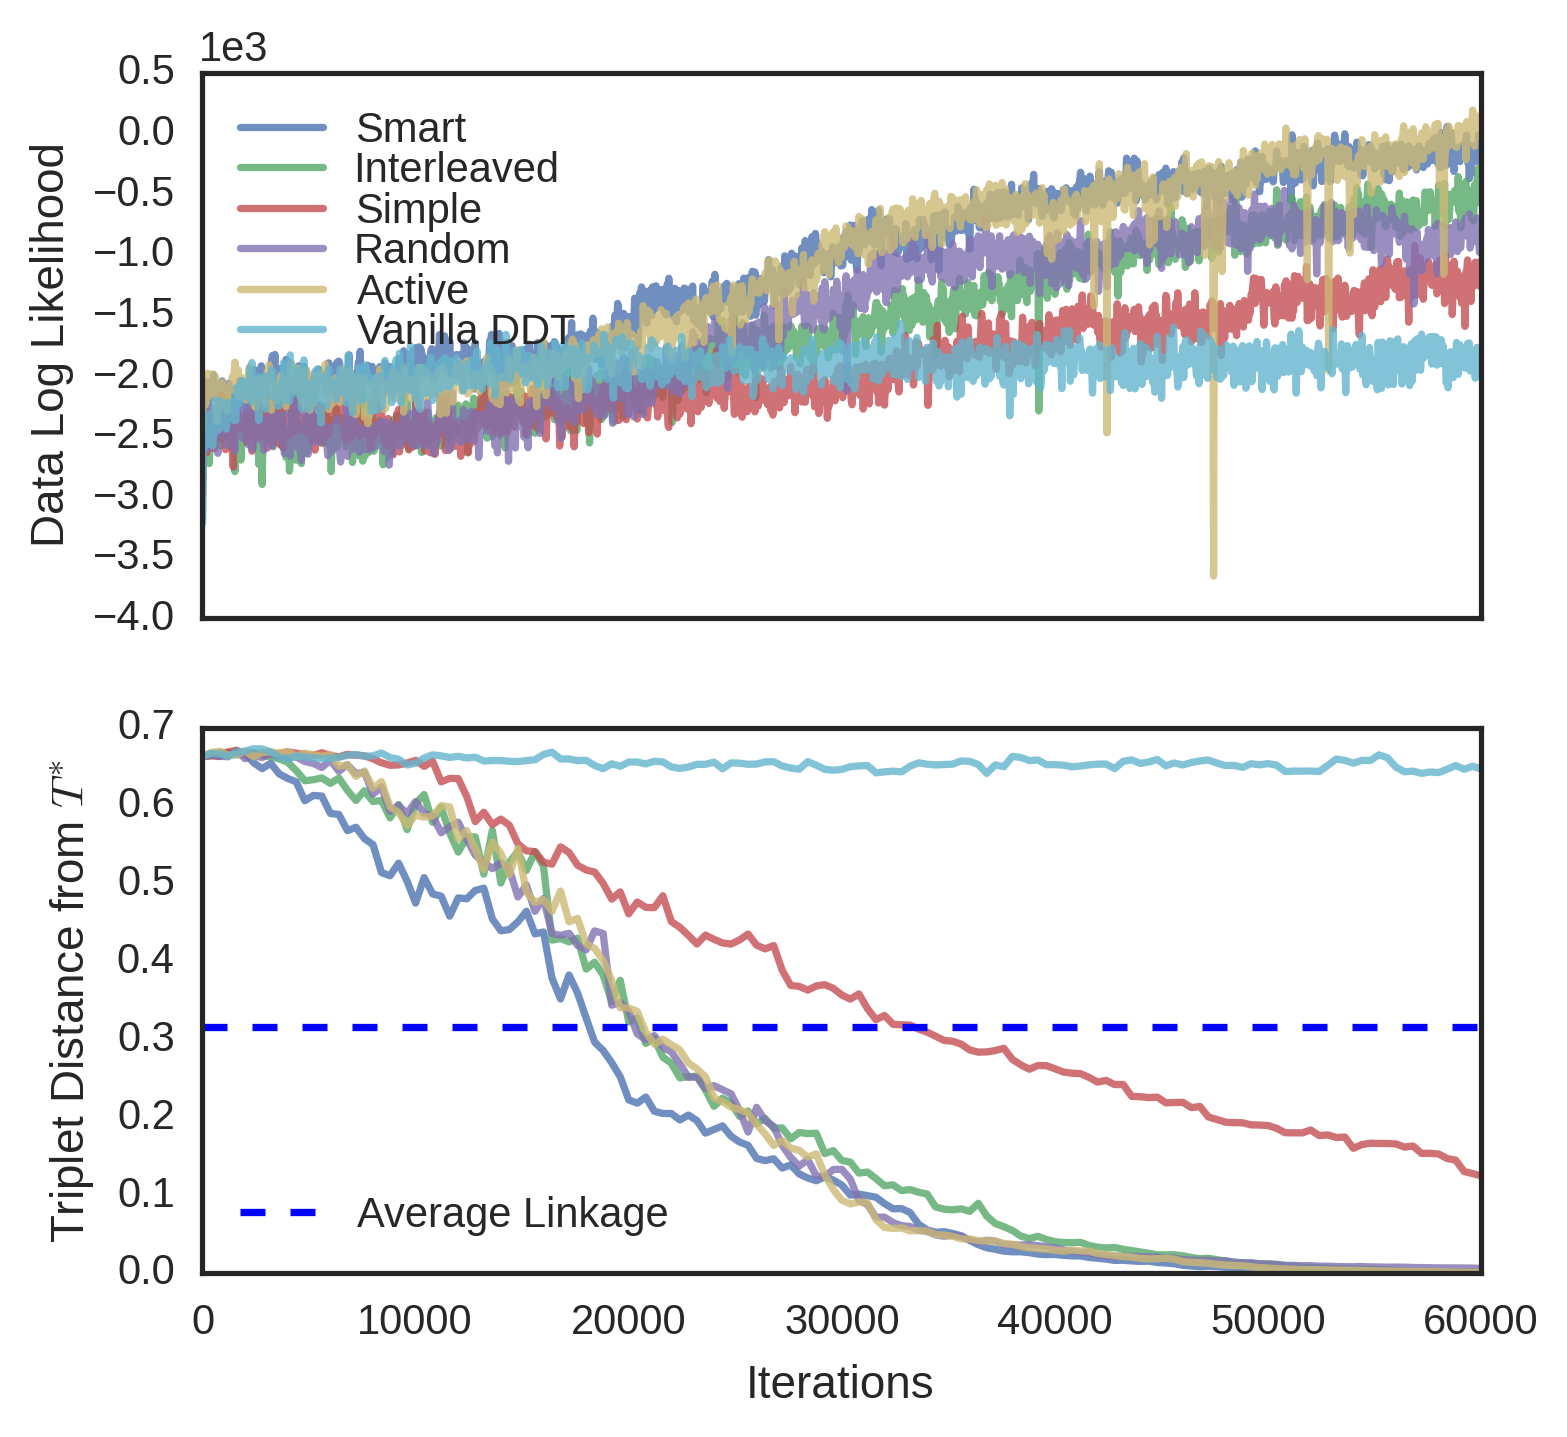
\includegraphics[frame, width=0.6\textwidth]{img/interactive}
    \caption{The results of interactive Bayesian hierarchical clustering
    on a dataset of zoo animals. Pictured are the
    data log likelihood and percentage of triplets
    satisfied for several subset querying methods. Source: \cite{Vikram2016}}
    \label{fig:ibhc}
  \end{figure}
\end{frame}
\section{Conclusion}

\begin{frame}{Summary}
  \begin{itemize}
    \item<1-> Bayesian hierarchical clustering (BHC) is a general framework
      in unsupervised learning that naturally handles
      ambiguity and uncertainty in data.
    \item<2-> BHC models can be decomposed into prior distributions
      on trees, and likelihood models. Tree priors
      can further be decomposed into
      coalescent and diffusion models.
    \item<3-> Inference in BHC can be performed
      with MCMC methods like Metropolis-Hastings
      using the subtree-prune and regraft move.
    \item<4-> BHC enables
      incorporating user interaction
      into hierarchical clustering.
  \end{itemize}
\end{frame}

\begin{frame}{Future work}
  \begin{itemize}
    \item<1-> \textbf{How can we improve on interactive Bayesian hierarchical clustering?}
      Robust constraints, more tree priors, other measures of variance
    \item<2-> \textbf{What is the effect of interaction in Bayesian problems?}
      constrained posterior distributions, complexity of inference
    \item<3-> \textbf{How can we extend interactive methods
      to other domains?} metric learning, deep learning,
      embeddings
  \end{itemize}
\end{frame}

\begin{frame}[standout]
Questions?
\end{frame}

\begin{frame}[allowframebreaks]{References}
  \bibliography{main}
  \bibliographystyle{unsrt}
\end{frame}

\end{document}
